\documentclass[12pt, oneside]{article}
\usepackage[letterpaper, margin=1in, headsep=0.5in]{geometry}
\usepackage[english]{babel}
\usepackage[utf8]{inputenc}
\usepackage{amsmath}
\usepackage{amsfonts}
\usepackage{amssymb}
\usepackage{tikz}
\usetikzlibrary{quotes, angles}
\usepackage{graphicx}
%\usepackage{pgfplots}
%\pgfplotsset{width=10cm,compat=1.9}
%\usepgfplotslibrary{statistics}
%\usepackage{pgfplotstable}
%\usepackage{tkz-fct}
%\usepackage{venndiagram}
\usepackage{multicol}

\usepackage{fancyhdr}
\pagestyle{fancy}
\fancyhf{}
\rhead{\thepage \\Name: \hspace{1.5in}.\\}
\lhead{BECA / Dr. Huson / 10.3 Geometry\\* 9 January 2019}

\renewcommand{\headrulewidth}{0pt}

\begin{document}
  You only have to solve some of the problems, as shown. For those, show your work, and check your answer.
  \begin{enumerate}
    \subsubsection*{Classwork: Word problem Wednesday}

  \item At college, the phone company charges \$25 for installation plus \$28 per month. The total you saved over the summer for service was \$137. How many months can you pay for?
  \begin{enumerate}
    \item Mark the text of the problem and then complete the values:\\[0.5cm]
    Starting point $= \rule{2cm}{0.15mm}$ \\[0.5cm]
    Rate of change $= \rule{2cm}{0.15mm}$ \\[0.5cm]
    Total $= \rule{2cm}{0.15mm}$ \\

    \item Write an equation for the problem of the form $y=mx+b$\\[3cm]

  \end{enumerate}

  \item An acting consultant charges \$75 for an initial meeting plus \$35 per hour for consulting work. Your uncle gave you \$300 for acting lessons. How many hours work can you afford?
  \begin{enumerate}
    \item Initial amount $= \rule{2cm}{0.15mm}$ \\[0.5cm]
    Rate of change $= \rule{2cm}{0.15mm}$ \\[0.5cm]
    Total $= \rule{2cm}{0.15mm}$ \\

    \item Write an equation for the problem of the form $y=mx+b$\\[1.5cm]
  \end{enumerate}

\newpage

  \item A cleaner charges \$65 per day plus \$18 per hour. If you allow \$200 for cleaning expenses, how many hours work can you tell the cleaner to expect?
  \begin{enumerate}
    \item Initial point $= \rule{2cm}{0.15mm}$ \\[0.5cm]
    Rate of change $= \rule{2cm}{0.15mm}$ \\[0.5cm]
    Total $= \rule{2cm}{0.15mm}$ \\

    \item Write an equation for the problem of the form $y=mx+b$\\[1.5cm]

  \end{enumerate}

  \item A DJ charges \$200 to play for a party plus \$120 per hour. The total for Mr. Odouard's college reunion party was \$740. How many hours did the band play?
  \begin{enumerate}
    \item Mark the text of the problem and then complete the values:\\[0.5cm]
    Starting point $= \rule{2cm}{0.15mm}$ \\[0.5cm]
    Rate of change $= \rule{2cm}{0.15mm}$ \\[0.5cm]
    Total $= \rule{2cm}{0.15mm}$ \\

    \item Write an equation for the problem of the form $y=mx+b$\\[1.5cm]
    \item Solve the equation for $x$ \vspace{3.5cm}
    \item Check the answer \vspace{2.5cm}
  \end{enumerate}

\newpage
\item Graph the line $y=\frac{2}{3} x -2$ after filling in the values in the blanks.\\[0.85cm]
      $y$-intercept $= \rule{2cm}{0.15mm}$ \\[0.5cm]
      Slope $= \rule{2cm}{0.15mm}$\\

\begin{center} %4 quadrant regents grid w T-Chart
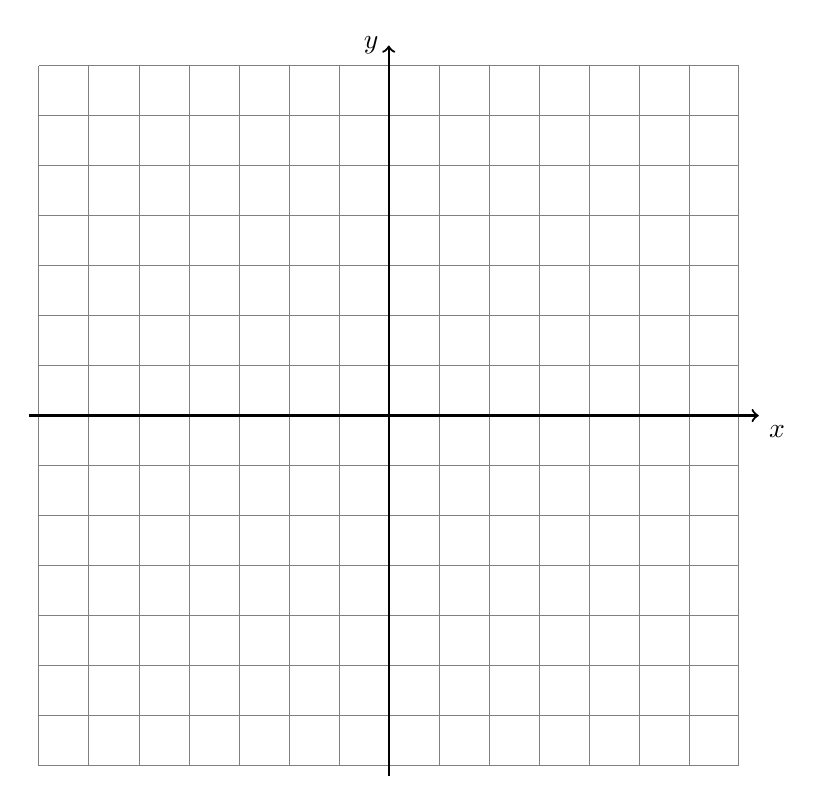
\begin{tikzpicture}[scale=.635]
  \draw [help lines] (-7,-7) grid (7,7);
  \draw [thick, ->] (-7.2,0) -- (7.4,0) node [below right] {$x$};
  \draw [thick, ->] (0,-7.2)--(0,7.4) node [left] {$y$};
\end{tikzpicture}
\end{center}

In the following two problems, solve for the value of $x$.
\begin{multicols}{2}
\item   $12=5x-x$ \vspace{3cm}
\item   $\frac{1}{4}(12-8x)=x$ %\vspace{3cm}
\end{multicols}

\newpage

In the following problems, write down the initial value and the slope. Solve for $y$ if necessary.
\begin{multicols}{2}
\item   $y=3x+3$ \vspace{3cm}
\item   $\frac{1}{4}(12-8x)=x$ %\vspace{3cm}
\end{multicols}

\newpage

\item
\begin{enumerate}
  \item For the function $y= |x-2|-1$, fill in the T-chart, plot the points, and draw the line.
    \begin{center} %4 quadrant regents grid w T-Chart
    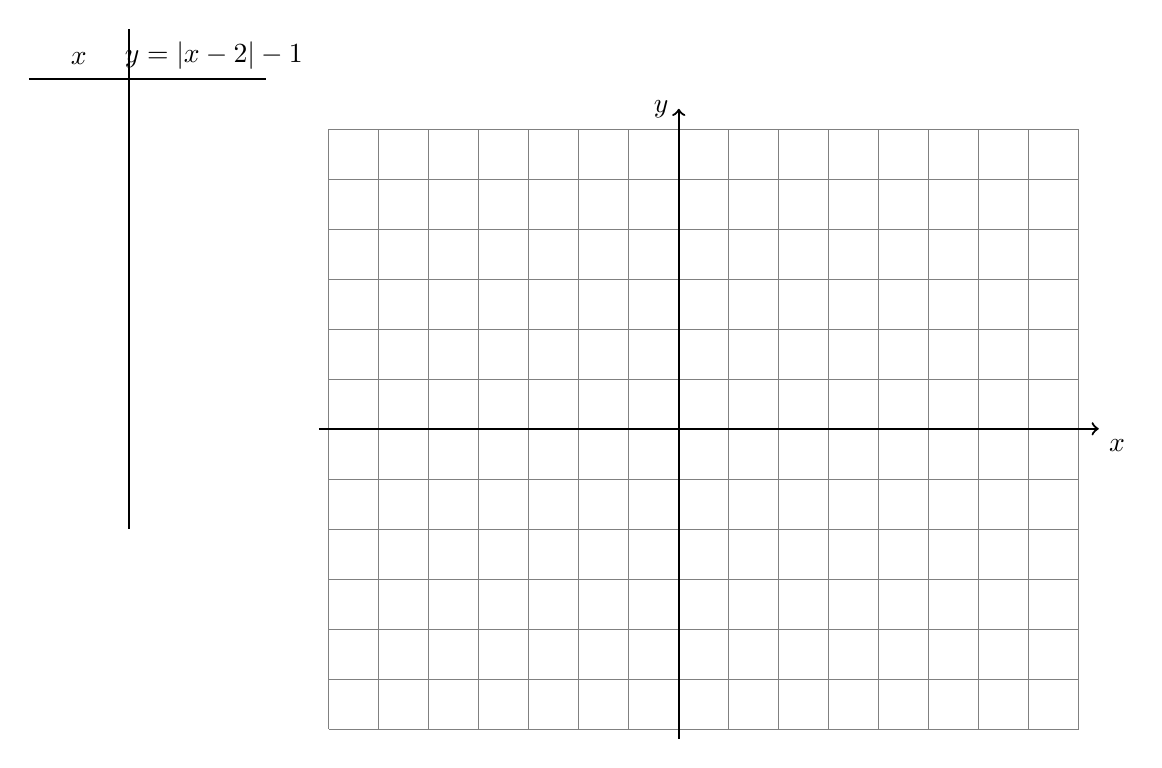
\begin{tikzpicture}[scale=.635]
      \draw [thick, -] (-11, -2)--(-11,8);
      \draw [thick, -] (-13,7)--(-8.25,7);
      \node at (-12,7.1) [above] {$x$};
      \node at (-9.3,7) [above] {$y= |x-2|-1$};
      \draw [help lines] (-7,-6) grid (8,6);
      \draw [thick, ->] (-7.2,0) -- (8.4,0) node [below right] {$x$};
      \draw [thick, ->] (0,-6.2)--(0,6.4) node [left] {$y$};
    \end{tikzpicture}
    \end{center}
    \item Write down the values for $x$ when $y=0$.\\[0.5cm]
    $x_1=$\\[0.5cm]
    $x_2=$\\[0.5cm]
    \item Circle the row for the $y$-intercept.
\end{enumerate}
\vspace{1cm}

In the following two problems, simplify by collecting like terms.
\begin{multicols}{2}
\item $3x^2-3x +5 -2x^2-x-4$ \vspace{3cm}
\item $4(a^2-2a +1) -3(a^2-a+2)$ \vspace{3cm}
\end{multicols}

\newpage

  \item After lunch on the day of the math test, Dr. Huson took 12 students for dessert. Some students wanted a snow cone, which cost \$2.50 each, and the others got cake, which cost \$3.00 each. The total cost was \$31.00. (Dr. Huson did not eat) How many students got each kind of dessert? \\[0.5cm]
  Use $x$ for the number of snow cone orders and $y$ for the number of cake orders.
  \begin{enumerate}
    \item Complete the table of costs below. (the first row is done as a hint)

    \renewcommand{\arraystretch}{1.6}
    \begin{center}
      \begin{tabular}{|c|c|r| r |r|}
      \hline
      $x$ & $y$ & cost for snow cones & cost for cake & total cost\\
      \hline
      0 & 12 & \$0.00 & \$36.00 & \$36.00 \\
      \hline
      2 & 10 &  &  &  \\
      \hline
      4 & 8 &  &  &   \\
      \hline
      6 & 6 &  &  &   \\
      \hline
      8 & 4 &  &  &   \\
      \hline
      10 & 2 &  &  &   \\
      \hline
      12 & 0 &  &  &   \\
      \hline
      \end{tabular}
    \end{center}

    \item Complete the two equations modeling the situation, one adding up to 12 people, the other adding up to \$31.00. \\[0.5cm]
    \hspace{6cm} $x  + y  = \rule{2cm}{0.15mm}$ \\[0.5cm]
    \hspace{3cm} $\rule{2cm}{0.15mm} \times  x + \rule{2cm}{0.15mm} \times y= \rule{2cm}{0.15mm}$

    \item Circle the row in the table that has the correct total. Write down how many students wanted ice cream and pie ($x$ and $y$).\\[0.5cm]
    \hspace{6cm} $x = \rule{2cm}{0.15mm}$ \\[0.5cm]
    \hspace{6cm} $y = \rule{2cm}{0.15mm}$

    \item Check your answer.
  \end{enumerate}

\newpage

  \begin{multicols}{2}
    Distribute
    \item $(x+2)(x+3)$ \vspace{2.5cm}
    \item $(x+4)(x+4)$

    Factor each expression
    \item $x^2+8x+7$ \vspace{2.5cm}
    \item $x^2+7x+10$
  \end{multicols}

\vspace{3cm}
Solve for the value of $x$.

\item   $5=\frac{1}{2}x+2x-10$ \vspace{3cm}


\item Given $f(x)=3x+5$. Simplify $f(3)$. \vspace{4cm}
\item Given $\displaystyle f(x)=-\frac{(6+3x)}{13}$. Simplify $f(-2)$.

\newpage

\end{enumerate}
\end{document}
